\documentclass{sig-alternate-05-2015}
\usepackage{paralist}
\usepackage{hyperref}

\begin{document}
\setcopyright{acmcopyright}
\conferenceinfo{ISSAC 2017}{July 25--28, 2017, Kaiserslautern, Germany}

\newtheorem{alg}{Algorithm}
\newtheorem{definition}{Definition}
\newtheorem{Assertion}{Assertion}

\makeatletter
\def\Ddots{\mathinner{\mkern1mu\raise\p@
\vbox{\kern7\p@\hbox{.}}\mkern2mu
\raise4\p@\hbox{.}\mkern2mu\raise7\p@\hbox{.}\mkern1mu}}
\makeatother

%\title{Hecke/Nemo: Number Theory packages for the Julia programming language}
\title{Hecke/Nemo: computer algebra and number theory packages for the Julia programming language}

\numberofauthors{4}
\author{
\alignauthor Claus Fieker\\
   \affaddr{TU Kaiserslautern}\\
   \affaddr{Fachbereich Mathematik, Postfach 3049,}\\
   \affaddr{67653 Kaiserslautern, Germany}\\
   \email{fieker@mathematik.uni-kl.de}
\alignauthor William Hart\\
   \affaddr{TU Kaiserslautern}\\
   \affaddr{Fachbereich Mathematik, Postfach 3049,}\\
   \affaddr{67653 Kaiserslautern, Germany}\\
   \email{goodwillhart@gmail.com}
\alignauthor Tommy Hofmann\\
   \affaddr{TU Kaiserslautern}\\
   \affaddr{Fachbereich Mathematik, Postfach 3049,}\\
   \affaddr{67653 Kaiserslautern, Germany}\\
   \email{thofmann@mathematik.uni-kl.de}
\and
\alignauthor Fredrik Johansson\\
   \affaddr{Inria Bordeaux \&}\\
   \affaddr{Institut de Math\'{e}matiques de Bordeaux} \\
   \affaddr{33400 Talence, France}\\
   \email{fredrik.johansson@gmail.com}
}

\maketitle

\begin{abstract}
We introduce two new packages, Hecke and Nemo, written in the Julia programming language
for computer algebra and number theory.
We demonstrate that high performance generic
algorithms can be implemented in Julia, without the need to resort to a low-level C
implementation. We also describe the various Julia wrappers of existing C/C++ libraries
such as Flint, Arb, Antic and Singular. We give examples of how to use Hecke and Nemo and discuss
some of the algorithms that we have implemented to provide high performance basic
arithmetic.
\end{abstract}


\section{Introduction}

Nemo is a computer algebra package for the Julia programming language. The eventual aim is
to provide highly performant Commutative Algebra, Number Theory and Group Theory routines.

Nemo consists of two parts. The first part consists of wrappers of specialised C/C++
libraries: Flint \cite{flint}, Arb \cite{Arb}, Antic \cite{Antic} and Singular
\cite{singular}.

The second part consists of implementations of generic algorithms and mathematical data
structures in the Julia language. So far the fully recursive constructions include
Univariate polynomial rings, Power series rings, Residue rings (modulo principal ideals),
Fraction fields, Matrices and more recently multivariate polynomials with a sparse
distributed representation.

\subsection{The Julia programming language}

Julia \cite{julia} is a sophisticated, modern programming language which is designe
to be both performant and flexible. It was written for technical computing with a
focus on numerics. However, it has found widespread use for many general purpose
applications, largely due to its innovative type system, dispatch mechanism, JIT
compilation and metaprogramming capabilities.

The first public version of Julia appeared in 2012. 

The benefits of Julia include:

\begin{itemize}
\item Familiar imperative syntax
\item Just-In-Time compilation
\item interactive console
\item Parametric types
\item Powerful metaprogramming facilities
\item Operator overloading
\item Multiple dispatch
\item Efficient native C interface
\item Experimental C++ interface
\item Dynamic type inference
\item Able to be embedded in C programs
\item High performance collection types (dictionaries, iterators, arrays, etc.)
\item Jupyter support (for web based notebooks)
\end{itemize}

\section{Modelling domains in Julia}

Julia provides two levels of types that we make use of abstract types and concrete types.
Concrete types are equivalent to the types that appear in languages such as Java, C or C++,
etc.

Abstract types can be thought of as collections of types. They are used when writing generic
functions that should work for any type in the given collection.

To write a generic function that accepts any type in a given collection of types, we first
create an abstract type. Then we create the individual concrete types that belong to that
abstract type. A generic function can then be constructed with a type parameter, T
say, similar to a template parameter in C++. The main difference is that we can specify
which abstract type our type parameter T must belong to.

In Julia, the symbol <: is used to specify that a given type belongs to a given abstract type.
For example the built-in Julia type Int64 for 64 bit machine integers belongs to the Julia
abstract type Integer.

Abstract types in Julia can form a hierarchy. For example, the Nemo.Field abstract type belongs
to the Nemo.Ring abstract type. An object representing a field in Nemo has type belonging to
Nemo.Field. But because we define the inclusion Nemo.Field <: Nemo.Ring, the type of such an
object also belongs to Nemo.Ring. This means that any generic function in Nemo which is designed
to work with ring objects will also work with field objects.

In Nemo/Hecke we distinguish between the elements of a field, and the field itself, and similarly
for and all other kinds of domains in Nemo. 

The diagram below shows the abstract type hierarchy in Nemo.

\begin{figure}[h]
\centering
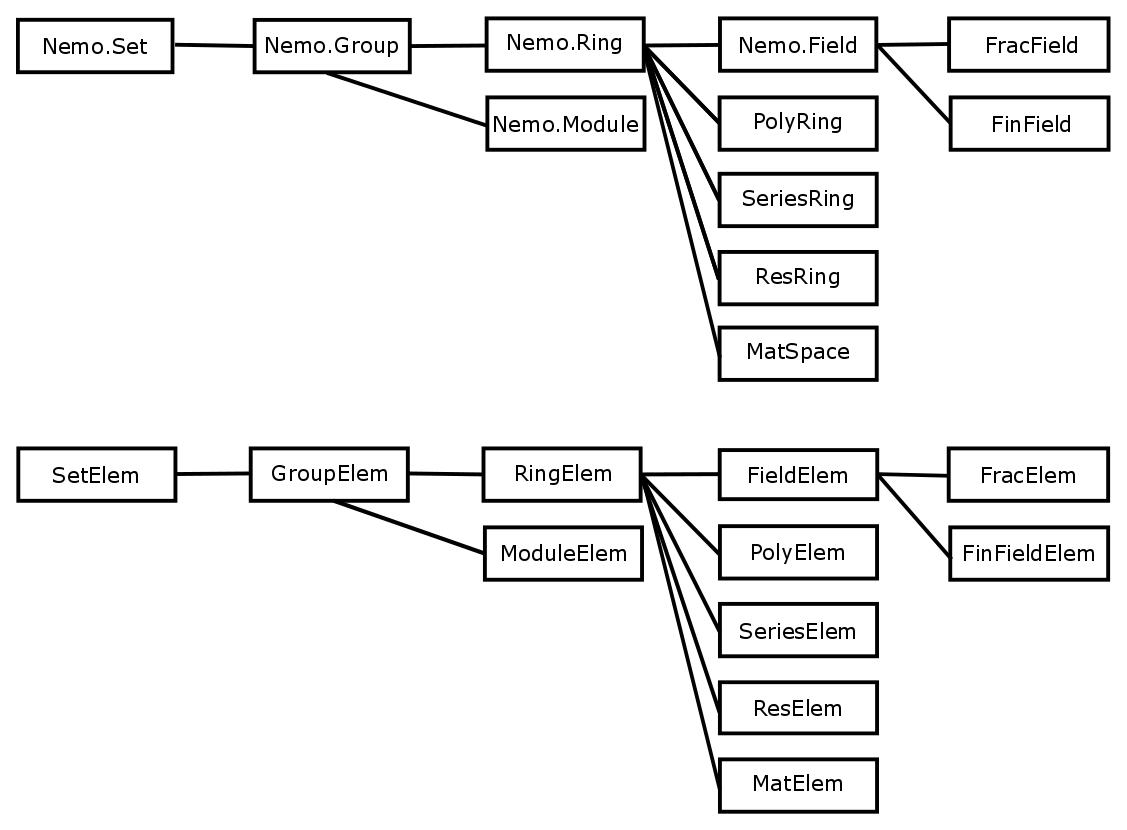
\includegraphics[scale=0.37]{types.png}
\caption{The Nemo abstract type hierarchy}
\end{figure}

Naively, one may expect that specific mathematical domains in Nemo/Hecke can be modeled as types
and their elements as objects of the given type. But there are various reasons why this is not a
good model.

As an example, consider the ring $R = \mathbb{Z}/n\mathbb{Z}$. If we were to model the ring $R$
as a type, then the type would need to contain information about the modulus $n$. This is not
possible in Julia if $n$ is an object, e.g. a multiprecision integer.

Putting such information in types is also not desirable. Julia dispatches on type, and each time
we call a generic function with different types, a new version of the function is compiled by the
JIT compiler. This would result in very poor performance if we were writing a multimodular
algorithm, say. In such an algorithm many rings $\mathbb{Z}/n\mathbb{Z}$ may be needed, and
recompilation would be triggered for each distinct $n$.

For this reason, the modulus $n$ needs to be attached to the elements of the ring, not to the type
associated with those elements.

The way we deal with this is to have special (singleton) objects, known as parent objects, that act
like types, but are in fact ordinary Julia objects. As ordinary objects, parents can contain
arbitrary information, such as the modulus in $\mathbb{Z}/n\mathbb{Z}$. Each element in the ring
$\mathbb{Z}/n\mathbb{Z}$ then contains a pointer to the relevant parent object.

This model of mathematical parent objects is taken from SageMath which in turn followed the Magma
computer algebra system.

Julia allows ordinary objects to be made callable. We make use of the facility to write coercions
and constructors for elements of mathematical domains in Nemo/Hecke. For example, the following
code constructs $a = 3 \pmod{7}$.

\begin{verbatim}
R = ResidueRing(ZZ, 7)
a = R(3)
\end{verbatim}

We also make use of the parent object system to encode information such as context objects needed
by C libraries. As Julia objects can have precisely the same bit representation as native C objects,
parent objects can be passed directly to C functions. Additional fields in these objects can safely
appended if it is desirable to retain more information at the Julia level than the C/C++ level. 

\section{Nemo: basic arithmetic in Julia}

\section{Hecke: algebraic number theory in Julia}

\section{Generic algorithms in Nemo}

\section{Specific algorithms in Nemo}

\subsection{Flint: number theory}

We envisioned Flint as a set of implementations for specific rings,
but now we realize that it makes sense to use it only for specific
rings where there is some trick

For example, there seems to be no need to have a Flint type for
matrices over $\left(\mathbb{Z}/n\mathbb{Z}\right)[x]$.

Julia has informed development - for example: don't want to just commit suicide
on bad input

Ground rings $\mathbb{Z}$, $\mathbb{Q}$, $\mathbb{Z}/n\mathbb{Z}$,
$\mathbb{F}_q, \mathbb{Q}_p$

dense univariate polynomials, dense matrices
and power series

some flint types require context objects; parent objects hold context objects

algorithms prototyped in Julia, then rewritten in C

showed the way for multivariate polynomials 

\subsection{Arb: arbitrary precision ball arithmetic}

Viable approaches to represent elements of $\mathbb{R}$ and $\mathbb{C}$
include floating-point approximations,
intervals, and lazy bit streams (e.g.\ using a finite-precision
approximation together with an exact symbolic DAG
to allow re-computing the approximation to higher precision).

Nemo includes wrapper code for Arb, which implements real numbers as
arbitrary-precision midpoint-radius intervals (balls) $[m \pm r]$
and complex numbers as rectangular boxes $[a \pm r_1]$ + $[b \pm r_2] i$.

While alternative implementations of $\mathbb{R}$ and $\mathbb{C}$
may be added to Nemo in the future, we envision Arb as a reasonable default,
and we have used it with good success (see Hecke).

For many computer algebra algorithms, the error analysis
necessary to guarantee correct results with floating-point arithmetic
becomes impractical to do by hand.
Interval arithmetic solves this problem by effectively making
error analysis automatic.

With arbitrary-precision interval arithmetic, a form of
coarse-grained lazy evaluation is possible: the user can
try a computation with some tentative precision $p$ and restart
with precision $2p$ if that fails. The precision can be set
optimally when a good estimate for the minimal
required~$p$ is available; that is, the intervals
can be used as if they were plain floating-point numbers, and the automatic
error bounds simply provide a certificate.

A lazy representation for single numbers would be more convenient in some
applications,
but also probably slower (and less space-efficient) due to storing DAGs.
Implementing lazy numbers on top of Arb in Julia
would be an interesting future project.

The midpoint-radius representation used by Arb is particularly efficient
at high precision,
since low precision is sufficient for the radii, which means that
speed and memory efficiency is close to the optimum possible
with plain arbitrary-precision floating-point arithmetic.
Like Flint, Arb systematically uses asymptotically fast algorithms
for operations such as polynomial multiplication, with tuning
for different problem sizes.


ArbField, AcbField

polynomials, matrices

also transcendental functions

\subsection{Antic: algebraic number fields}

\subsection{Singular: commutative algebra}

\section{Future directions}

\section{Acknowledgement}


\begin{thebibliography}{99}

\bibitem{magma}
J. J. Cannon, W. Bosma (Eds.) {\em Handbook of Magma Functions}, Edition 2.13 (2006)

\bibitem{mca} 
J. von zur Gathen and J. Gerhard. {\em Modern Computer Algebra}. Cambridge University Press, 1999.

\bibitem{flint}
W. Hart, F. Johansson and S. Pancratz. {\em FLINT}, open-source C-library. \url{http://www.flintlib.org}

\bibitem{arb}
F. Johansson. {\em Arb}, open-source C-library. \url{http://arblib.org}

\bibitem{ntl}
V. Shoup {\em NTL}, open-source C++ library. \url{http://www.shoup.net/ntl/}

\bibitem{sage}
W. Stein {\em SAGE Mathematics Software}.  \url{http://www.sagemath.org}

\bibitem{julia} J. Bezanson, A. Edelman, S. Karpinski and V. B. Shah. {\em Julia: A fresh approach to numerical computing}. \url{https://arxiv.org/abs/1411.1607}

\bibitem{singular} W. Decker, G. M. Greuel, G. Pfister and H. Sch\"onemann. {\em Singular} --- A computer algebra system for polynomial computations. \url{http://www.singular.uni-kl.de}

\end{thebibliography}
\end{document}
